%\chapter{Introduction to Linear Programming}
\chapter{Computational Complexity for Linear Programming}

\section{A case study}
Suppose we aim to find a shortest path on a directed network, from the source node $s$ to the sink node $t$. The network is supposed to be $\mathcal{N}=(V,E;w)$, where $V=\{v_1,\dots,v_n\}$ is the set of nodes, $E$ is the set of edges, and $w$ is the vectors of weights, i.e., $w_{ij}$ denotes the weight on the edge $(v_i,v_j)$.

We need to input this instance into the computer. One way is to use the \emph{node-arc} incidence matrix:
\[
a_{ij}=\left\{
\begin{aligned}
-1,&\quad\text{if $v_i$ is the head of arc $e_j$}\\
0,&\quad\text{if $v_i$ is not related to arc $e_j$}\\
+1,&\quad\text{if $v_i$ is the tail of arc $e_j$}
\end{aligned}
\right.
\]
\paragraph{Input size of a problem}
\begin{enumerate}
\item
Suppose $|V|=n$ and $|E| = m$, then inputting the matrix $A$ requires to touch the keyboard $mn+2m$ times.
\item
To tell the vector $w$ into computer, we need $w$ to be \emph{integer-valued} (since otherwise the problem will be much more difficult. question: do $w$ need to be positive?). Typing $w_{ij}$ requires at most $\lfloor\log_2(|w_{ij}|+1)\rfloor+1$ bits. Therefore typing the vector $w$ requires totally 
\[
\sum_{(v_i,v_j)\in E}\lfloor\log_2(|w_{ij}|+1)\rfloor+|E|\text{ bits}
\]
\item
Therefore, the input-length (size) of this problem is
\[
L = mn + 3m + \sum_{(v_i,v_j)\in E}\lfloor\log_2(|w_{ij}|+1)\rfloor.
\]
\end{enumerate}

\paragraph{The Running Time Complexity}
It's logical that the total amount of perations required by an algorithm to solve this problem is \emph{dependent} on $L$.

Consider applying the \emph{Dijkstra} algorithm to find the shortest path from the source node $s$ to the sink node $t$. 
Define a relevant working set $S$ that contains all the nodes with \emph{known shortest distance} to $t$. Initially $S=\{t\}$.
At each iteration, by \emph{dynamic programming principle}, one node is identified to be in $S$ after at most $\mathcal{O}(|V|)$ comparisions. 
Therefore, the overall computational complexity is $\mathcal{O}(|V|^2)$.

\section{Computational Complexity}
\paragraph{Polynomial Time Algorithm}
If an algorithm solves a combinatorial problem with input size $L$ with total number of operations no more than a polynomial of $L$, then it is called a \emph{polynomial-time} algorithm.

The Dijkstra algorithm requires no more than $\mathcal{O}(L^2)$ (question: $\mathcal{O}(L)$ or $\mathcal{O}(L^2)$?) operations to terminate, and therefore it is a polynomial-time algorithm. 

However, there are many combinatorial problems for which no polynomial time algorithms are known, e.g., the longest path problem, the Hamitonian circle problem, the maximum cut, and many more.

\subsection{P $\&$ NP}
\begin{definition}[NP problem]
If a combinatorial decision problem with input size $L$ is such that:
\begin{quotation}
if the answer to the problem is yes, then a yes-certificate exists and the length (size) of which is polynomial in $L$.
\end{quotation}
then we call the problem is \emph{NP}.
\end{definition}

\begin{definition}[co-NP problem]
If a combinatorial decision problem with input size $L$ is such that:
\begin{quotation}
if the answer to the problem is no, then a no-certificate exists and the length (size) of which is polynomial in $L$.
\end{quotation}
then we call the problem is \emph{co-NP}.
\end{definition}

\begin{definition}[P problem]
A \emph{polynomially solvable} problem is called to be \emph{P}.
\end{definition}

It's clear that $P\subseteq NP$ and $P\subseteq \emph{co-NP}$. 

\begin{definition}[NP-Complete problem]
The problem in NP such that any other problem in NP can be reduced to it is called to be \emph{NP-Complete}.
\end{definition}

It's \emph{strongly believed (haven't shown)} that NP-Complete problems are not in P.

\subsection{Dimensions and Parameters}

A decision problem typically involves \emph{dimension} and the \emph{parameters} of the problem, though thery are mixed in the definition of input-length $L$.
\begin{itemize}
\item
In the case study, $n=|V|$ and $m = |E|$ are known to be the problem dimensions, and the weight $w$ is known as the problem parameter.
\item
For the linear programming with integer-valued parameters
\[
\begin{array}{ll}
\max&\sum_{j=1}^nc_jx_j\\
\mbox{such that}&\sum_{j=1}^na_{ij}x_j\le b_i,\quad i=1,\dots,m\\
&x_j\ge0,\quad j=1,\dots,n
\end{array}
\]
the problem dimension would be $m$ and $n$, and the input-length is
\[
L = mn+m+n+\sum_{j=1}^n\lfloor
\log_2(|c_{j}|+1)
\rfloor
+
\sum_{i=1}^m\lfloor
\log_2(|b_i|+1)
\rfloor
+
\sum_{i=1}^m\sum_{j=1}^n\lfloor
\log_2(|a_{ij}+1|)
\rfloor.
\]
\end{itemize}

\subsection{Other terminologies}

\begin{definition}[Weak $\&$ Strong Polynomial Time Algorithms]
If a \emph{polynomial-time} algorithm requires number of operations to be \emph{polynomial} in dimensions, then the algorithm is called the \emph{strongly polynomial}, otherwise it is only \emph{weakly polynomial}
\end{definition}
\begin{remark}
Note that the input size of a problem defines the polynomial time, and the dimension specializes the strong $\&$ weak polynomial time.
The number of operations is different from the number of \emph{bit} operations.
The Dijkstra algorithm is strongly polynomial.
\end{remark}

\begin{definition}[Weak $\&$ Strong NP-Completeness]
If an \emph{NP-complete} is such that
\emph{even when it is restricted to be the case where all the parameters are constants}, it still remains to be \emph{NP-complete}, then it is called \emph{strongly NP-Complete}, otherwise it is called \emph{weakly NP-complete}.
\end{definition}

Example: the 2-partition problem is weakly NP-complete; the Hamiltonian circle problem is strongly NP-complete.

\begin{definition}
If a decision version of the problem is \emph{NP-complete} or \emph{co-NP-complete}, then the problem is called \emph{NP-Hard}.
\end{definition}

For example, the travelling salesman (TRS) problem is NP-Hard.

\section{Complexity of Linear Programming}

\subsection{LP is both NP and Co-NP}
The decision version of LP is: does there exists $\bm x$ satisfying
\[
\begin{array}{lll}
\bm c\trans\bm x\ge\bm v,
&
\bm{Ax}\le\bm b,
&
\bm x\ge0?
\end{array}
\]
\begin{enumerate}
\item
If the answer is yes, then a certificate is such $\bm x$, whose size can be bounded by a polynomial of the input-length.
\item
If the answer is no, then the above system is infeasible. By Farkas Lamma, there exists $y_0\ge0$ and $\bm y\ge0$ such that 
\[
\begin{array}{ll}
-y_0\bm c\trans + \bm y\trans\bm A\ge0,
&
-y_0\bm v + \bm y\trans\bm b<0.
\end{array}
\]
In this case, the size of no-certificate $(y_0,\bm y)$ can be bounded by a polynomial of the input-length.
\end{enumerate}

\subsection{Is LP in P?}

In the complexity theory, we believe that $P\subsetneqq NP$, i.e., $\text{P} \ne \text{NP-Complete}$ and $\text{NP}\cap\text{Co-NP}  =\text{P}$. Therefore, a natural question arises: Is linear programming in P? The answer is no, but the simplex method is \emph{not} a polynomial time algorithm. Let's study an example first.

\paragraph{The Klee-Minty Example (n=3)}
\begin{subequations}
Consider solving a LP using the Largest Coefficient Rule:
\begin{equation}
\begin{array}{ll}
\max&100x_1+10x_2+x_3\\
\mbox{such that}&x_1\le 1\\
&20x_1+x_2\le 100\\
&200x_1+20x_2+x_3\le10000\\
&x_1\ge0,x_2\ge0,x_3\ge0
\end{array}
\end{equation}
We can find its dictionary:
\begin{equation}
\begin{aligned}
\bm{x_4}&=1-x_1\\
x_5&=100-20x_1-x_2\\
x_6&=10000-200x_1-20x_2-x_3\\
z&=\bm{100x_1}+10x_2+x_3
\end{aligned}
\end{equation}
If we choose the variable with largest coefficient to enter the basis, i.e., $x_1$, we obtain:
\begin{equation}
\begin{aligned}
x_1&=1-x_4\\
\bm{x_5}&=80+2-x_4-x_2\\
x_6&=9800 +200x_4-20x_2-x_3\\
z&=100-100x_4+\bm{10x_2}+x_3
\end{aligned}
\end{equation}
If we choose the variable with largest coefficient to enter the basis, i.e., $x_2$, we obtain:
\begin{equation}
\begin{aligned}
\bm{x_1}&=1-x_4\\
x_2&=80+20x_4-x_5\\
x_6&=8200-200x_4+20x_5-x_3\\
z&=900+\bm{100x_4}-10x_5+x_3
\end{aligned}
\end{equation}
If we choose the variable with largest coefficient to enter the basis, i.e., $x_4$, we obtain:
\begin{equation}
\begin{aligned}
x_4&=1-x_1\\
x_2&=100-20x_1-x_5\\
\bm{x_6}&=8000+200x_1+20x_5-x_3\\
z&=1000-100x_1-10x_5+\bm{x_3}
\end{aligned}
\end{equation}
If we choose the variable with largest coefficient to enter the basis, i.e., $x_3$, we obtain:
\begin{equation}
\begin{aligned}
\bm{x_4}&=1-x_1\\
x_2&=100-20x_1-x_5\\
x_3&=8000+200x_1+20x_5-x_6\\
z&=9000+\bm{100x_1}+10x_5-x_6
\end{aligned}
\end{equation}
If we choose the variable with largest coefficient to enter the basis, i.e., $x_1$, we obtain:
\begin{equation}
\begin{aligned}
x_1&=1-x_4\\
\bm{x_2}&=80+20x_4-x_5\\
x_3&=8200-200x_4+20x_5-x_6\\
z&=9100-100x_4+\bm{10x_5}-x_6
\end{aligned}
\end{equation}
If we choose the variable with largest coefficient to enter the basis, i.e., $x_5$, we obtain:
\begin{equation}
\begin{aligned}
\bm{x_1}&=1-x_4\\
x_5&=80+20x_4-x_2\\
x_3&=9800+200x_4-20x_2-x_6\\
z&=9900+\bm{100x_4}-10x_2-x_6
\end{aligned}
\end{equation}
If we choose the variable with largest coefficient to enter the basis, i.e., $x_4$, we obtain:
\begin{equation}
\begin{aligned}
x_4&=1-x_1\\
x_5&=100-20x_1-x_2\\
x_3&=10000-200x_1-20x_2-x_6\\
z&=10000-100x_1-10x_2-x_6
\end{aligned}
\end{equation}
After total 7 simplex pivot steps, we get the optimal solution. This process is mazy, while it only contains 3 variables.
\end{subequations}

\paragraph{General Case}
Consider the general Klee-Minty example:
\[
\begin{array}{ll}
\max&\sum_{j=1}^n10^{n-j}x_j\\
\mbox{such that}&2\sum_{j=1}^{i-1}10^{i-j}x_j+x_i\le100^{i-1},\quad i=1,\dots,n\\
&x_j\ge0,\quad j=1,\dots,n
\end{array}
\]
Its input-length (in digits) should be:
\begin{align*}
&\sum_{j=1}^n(n-j-1)+\sum_{i=1}^n(2(i-1) +1)+\sum_{i=1}^n\left(\sum_{j=1}^{i-1}(i-j-1)+1\right)\\
&=\frac{n^3+12n^2+5n}{6}\\
&=\mathcal{O}(n^3)
\end{align*}
Let the slack variables be:
\[
s_i:=100^{i-1}-2\sum_{j=1}^{i-1}10^{i-j}x_j-x_i,\quad i=1,\dots,n
\]
One can show that in every feasible basis, either $x_i$ or $s_i$ must be in the basis, $i=1,\dots,n$, which implies that there are $2^n$ feasible basis in total.

If applying the largest coefficient pivot rule, then after $2^{n-1}-1$ iterations, the last row reads
\[
z=10\left(100^{n-2}-\sum_{j=1}^{n-2}10^{n-1-j}x_j-s_{n-1}\right)+x_n
\]
After further $2^{n-1}$ iterations, the last row reads
\[
z=90\cdot100^{n-2}+10\left(\sum_{j=1}^{n-2}10^{n-1-j}x_j+s_{n-1}\right)-s_n
\]
After further $2^{n-1}$ iterations, the last row reads
\[
z=100^{n-1}-\sum_{j=1}^{n-1}10^{n-j}x_j-s_n,
\]
which corresponds to an optimal basic solution.
\begin{remark}
Since the total number of pivot steps for the Klee-Minty example is $\mathcal{O}(2^n-1)$ for a problem whose input-length is $\mathcal{O}(n^3)$, it shows that in the worst case the simplex method with the largest coefficient pivot rule is exponential.

Most other conceivable simplex pivot rules all admit similar exponential examples. However, it remains open that whether we can find a special simplex pivot rule that is polynomial even in the worst case.
\end{remark}

The following figure shows the Geometric process for the Klee-Minty example with $n=3$, and here $(s_1,s_2,s_3) = (x_1,100x_2,10000x_3)$:
\begin{figure}[H]
\centering
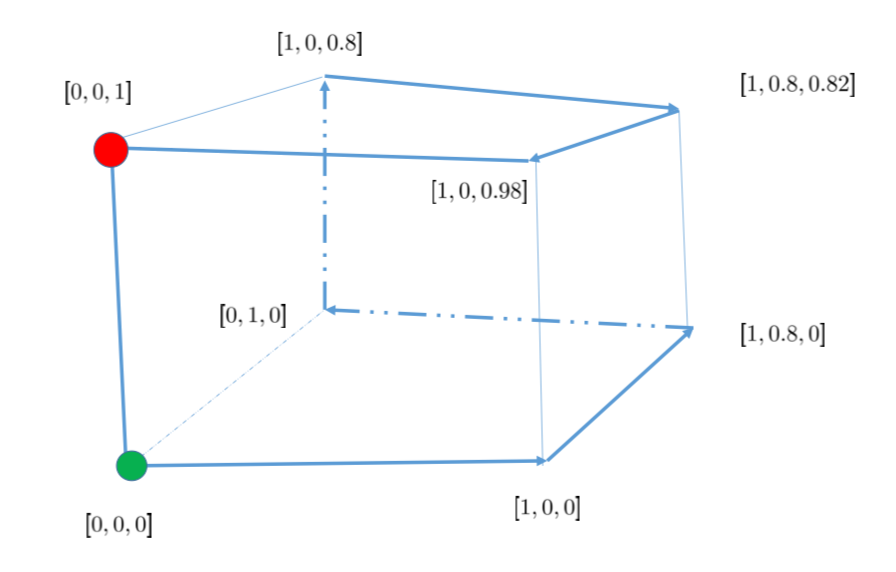
\includegraphics[width=0.9\textwidth]{Third_lecture/p_1}
\caption{A Geometric Picture for the Klee-Minty example with $n=3$}
\end{figure}








